% The quantum algorithm from candidate list to verification. The column nodes adapt
% fig3_tournament.tex; the verification box follows fig1_column.tex.
\documentclass[tikz,border=0pt]{standalone}
% Shared TikZ style for the figures of docs/exposition.md.
% Palette and bit cells follow docs/figures/expert_column.tex.
\usepackage{amsmath,amssymb}
\usetikzlibrary{arrows.meta,positioning,calc,decorations.pathreplacing}
\definecolor{one}{RGB}{226,232,240}
\definecolor{zero}{RGB}{40,40,40}
\definecolor{win}{RGB}{176,58,46}
\definecolor{addr}{RGB}{40,90,150}
\definecolor{lose}{RGB}{110,110,110}
\tikzset{
  bit/.style={draw=black!60, minimum width=4.4mm, minimum height=4.4mm,
              inner sep=0pt, font=\scriptsize},
  onebit/.style={bit, fill=one},
  zerobit/.style={bit, fill=zero, text=white},
  cell/.style={draw=black!50, fill=white, minimum width=10mm,
               minimum height=4.2mm, inner sep=0pt, font=\scriptsize},
  >={Stealth[length=2.2mm]}}

% \boardcolumn{name}{x}{b1}{b2}{b3}{b4}{address text}
% Draws X_name as four bits at height 0 starting at x, the address inputs
% below, and the four cells 00,01,10,11 named <name>c00 ... <name>c11.
\newcommand{\boardcolumn}[7]{%
  \node[anchor=east, font=\small] at (#2-0.05,0) {$X_{#1}$};
  \foreach \c/\b in {1/#3,2/#4,3/#5,4/#6} {
    \ifnum\b=0
      \node[zerobit] (x#1-\c) at (#2+0.46*\c-0.23,0) {0};
    \else
      \node[onebit] (x#1-\c) at (#2+0.46*\c-0.23,0) {1};
    \fi}
  \node[font=\scriptsize, align=center, addr, anchor=north] (adr#1)
    at (#2+0.92,-0.38) {#7};
  \foreach \s/\k in {00/0,01/1,10/2,11/3} {
    \node[cell] (#1c\s) at (#2+0.92,-1.62-0.5*\k) {$B_{#1,\s}$};}
}

\usetikzlibrary{backgrounds}
\begin{document}
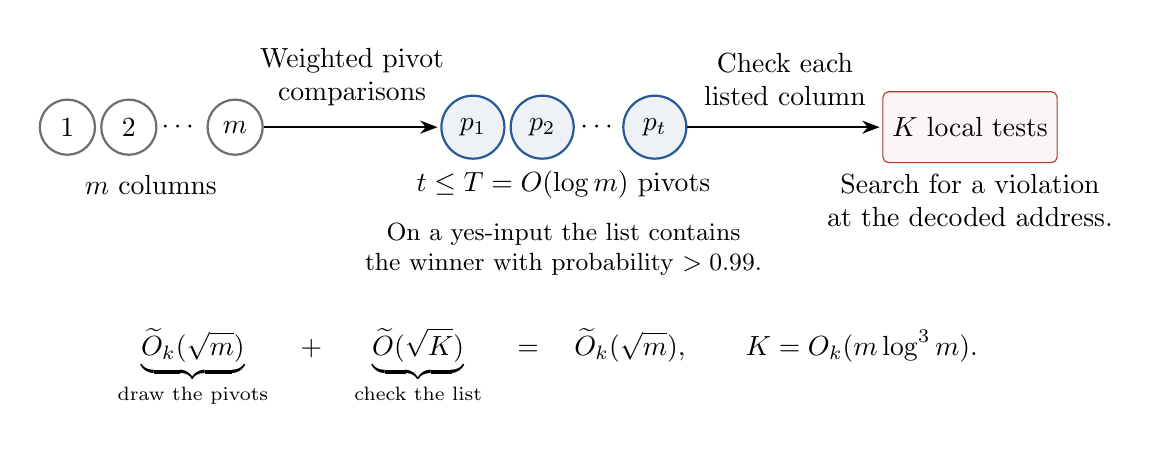
\begin{tikzpicture}[
  show background rectangle, background rectangle/.style={fill=white},
  inner frame sep=4pt, font=\normalsize,
  col/.style={circle, draw=lose, thick, minimum size=7mm, inner sep=1pt,
              fill=white},
  listed/.style={col, draw=addr, fill=addr!8, minimum size=8mm},
  flow/.style={->, thick, shorten >=1pt}]
% The pivot list is the only object passed to the expensive verifier.
\node[col] at (0,0) {$1$};
\node[col] at (0.78,0) {$2$};
\node at (1.43,0) {$\cdots$};
\node[col] (last) at (2.13,0) {$m$};
\node at (1.06,-0.73) {$m$ columns};
\node[listed] (first) at (5.15,0) {$p_1$};
\node[listed] at (6.03,0) {$p_2$};
\node at (6.75,0) {$\cdots$};
\node[listed] (end) at (7.46,0) {$p_t$};
\node at (6.30,-0.73) {$t\le T=O(\log m)$ pivots};
\draw[flow] (last.east) -- node[above=4pt, align=center] {Weighted pivot\\comparisons} (first.west);
\node[draw=win, fill=win!5, rounded corners=2pt, align=center,
      minimum height=9mm, anchor=west] (check) at (10.35,0) {$K$ local tests};
\draw[flow] (end.east) -- node[above=4pt, align=center] {Check each\\listed column} (check.west);
\node[align=center] at (check |- 0,-0.93) {Search for a violation\\at the decoded address.};
\node[align=center, font=\small] at (6.30,-1.55)
  {On a yes-input the list contains\\the winner with probability $>0.99$.};
\node at (6.10,-3.05) {$\displaystyle
  \underbrace{\widetilde O_k(\sqrt m)}_{\text{draw the pivots}}
  \quad+\quad
  \underbrace{\widetilde O(\sqrt K)}_{\text{check the list}}
  \quad=\quad\widetilde O_k(\sqrt m),
  \qquad K=O_k(m\log^3m).$};
\end{tikzpicture}
\end{document}
